\documentclass{report}
\usepackage[utf8]{inputenc}
\usepackage{graphics}
\graphicspath{ {./images/} }
\usepackage{multicol}

% width,height
\usepackage[a4paper, total={7in, 10in}]{geometry}

\title{IOT based smart surveillance system}
\author{Muhammad Waseem H}
\date{January 21, 2023}

\begin{document}

    \begin{titlepage}
    \centering
        \vspace*{2cm}
        \Huge
        \textbf{IoT-based Smart Surveillance System}
        
        \vspace*{0.6cm}
        \Large
        \textit{Assignment}
        
        \normalsize
        \vspace*{1.5cm}
        Muhammad Waseem H\\
        \vspace{0.2cm}
        21011101078\\
        \vspace{0.2cm}
        AI-DS B\\
        
        \vfill
        
        %\large
        
        %\begin{figure}[h]   % Figure Environment
        %    \centering
        %    \includegraphics[width = 6cm]{logo2}  % including the picture
        %    \caption{Muhammad Waseem H}
        %    \label{fig:my_image}
        %\end{figure}
        
        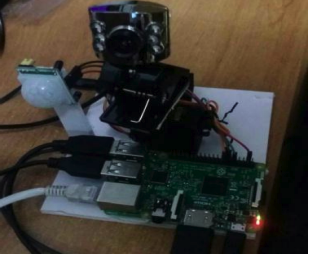
\includegraphics{kand}\\
        
        \vfill
        
        %\includegraphics[scale=0.5]{logo}
        
        
\includegraphics{logo3}\\
        Computer Science and Engineering\\
        Shiv Nadar University, Chennai\\
        21 January, 2023
        \vspace*{1cm}
    
\end{titlepage}
    
    \begin{center}
        \section*{IoT in Surveillance}
    \end{center}
\setlength{\columnsep}{1.0cm}
    \large
    \section*{Introduction}
    In recent years, the Internet of Things (IoT) has seen rapid growth and development. An IoT-based security system allows users to remotely monitor activity and capture images of their choosing. This is facilitated by an Android application, which sends notifications to users when motion is detected by PIR sensors and enables them to view images from a remote location. The system can operate in both automatic and manual modes, with notifications only sent in automatic mode to minimize interruptions. The system also allows users to remotely control and adjust the position of a camera connected to a Raspberry Pi device and capture new images
    
\begin{multicols}{1}    
    \section*{Application}
    The author describes a proposed security system that aims to improve security, flexibility, and efficiency compared to previous systems. The system includes an Android application, which allows the user to receive notifications of detected motion and view live streaming of the location from a remote location. It includes a Raspberry Pi device with a connected camera and PIR sensors, which detect motion and capture images. The system is designed to work in two modes, automatic and manual, with notifications only sent in automatic mode to minimize interruptions. The system also allows the user to remotely control and adjust the position of the camera, and capture new images. It involves a python script that directs the Raspberry Pi to send push notifications to the user when motion is detected. The system also includes a cloud platform for storing and processing the data generated by the device. The system also includes an Android application that the user installs in order to receive notifications from the cloud.
    
    \section*{Architecture}
    In the proposed paper the author uses hybrid architecture. In a hybrid architecture, there is a central hub or server that acts as the main point of communication between all the IoT devices. This central hub is responsible for managing and coordinating the devices, as well as processing and analyzing the data that is generated by the devices. However, unlike a fully centralized architecture, the devices in a hybrid architecture are also able to communicate directly with each other, forming a network of devices. This allows for a more distributed and resilient system, where the devices can still function even if the central hub is unavailable.

    This type of architecture allows to take advantage of the simplicity and ease of management of a centralized architecture and the scalability and resilience of a decentralized architecture.
    
    Hybrid architecture is particularly useful in large-scale, complex IoT systems where a mix of centralized and distributed control is needed. This can be especially useful in industrial, smart home, and smart cities environments, where the ability to process and analyze data locally, as well as remotely, is important.
    
    The key aspect of the hybrid architecture is that it allows for a balance between the centralized and decentralized elements, depending on the specific needs of the system. This allows for a more flexible and adaptable system that can be tailored to the specific requirements of the application.
    
    \section*{Protocol}
    The protocol was not clearly mentioned, but it is mentioned that the system uses a cloud platform, which is used to store, process and analyze the data generated by the device. The Android application is used to register the device and receive notifications from the cloud. These functionalities are commonly used in IoT systems and it is possible that the system uses HTTP protocol for communication between the device and the cloud.

    HTTP (Hypertext Transfer Protocol) is a standard protocol for communication on the internet. It is widely used in IoT systems to send and receive data between devices and servers. HTTP is a request-response protocol, which means that the client (e.g., the Raspberry Pi device) sends a request to the server (e.g., the cloud platform), and the server responds with the requested data. The HTTP protocol is based on the Transmission Control Protocol (TCP) and is a reliable and widely supported protocol for communication in IoT systems.
\end{multicols}
\end{document}
